% Fig 2.3 -- pmf of a fair die with the threshold x = 3.4 (web-original
%             figure, no manuscript tikzpicture; redrawn 2026-08-02 to
%             replace the hand-written SVG, which carried Chinese labels)
% Same x range and tick scheme as Fig 2.4 (dice-cdf-jump.tex).
\documentclass[tikz,border=2pt]{standalone}
\usepackage{amsmath}
\usepackage{amssymb}
\usepackage{xcolor}
\usetikzlibrary{arrows.meta}
\newcommand{\sssig}{\scriptscriptstyle}

\definecolor{journalink}{HTML}{1F1C18}
\definecolor{journalmuted}{HTML}{8A7F72}
\definecolor{journalaccent}{HTML}{9C2D2D}

\begin{document}
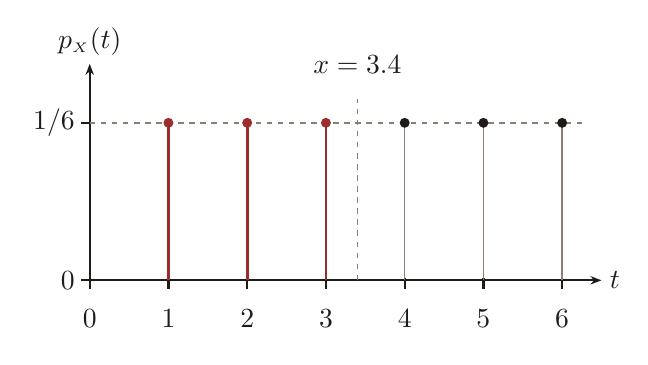
\begin{tikzpicture}[
  x=1cm,
  y=1cm,
  every node/.style={font=\normalsize, journalink},
  axis/.style={journalink, line width=0.8pt, -{Stealth[length=4pt]}},
  tick/.style={journalink, line width=0.8pt},
  guide/.style={journalmuted, line width=0.5pt, dash pattern=on 2pt off 2pt},
  stemin/.style={journalaccent, line width=1.0pt},
  stemout/.style={journalmuted, line width=0.5pt},
  solidpt/.style={circle, fill=journalink, inner sep=0pt, minimum size=3.6pt},
  accentpt/.style={circle, fill=journalaccent, inner sep=0pt,
                   minimum size=3.6pt}
]
  % ---- axes ----
  \draw[axis] (0,0) -- (6.5,0);
  \draw[axis] (0,0) -- (0,2.75);

  % ---- x ticks (same scheme as Fig 2.4) ----
  \foreach \x in {0,1,2,3,4,5,6}{
    \draw[tick] (\x,0.035) -- (\x,-0.106);
    \node[anchor=north] at (\x,-0.25) {$\x$};
  }

  % ---- y ticks: y=2 corresponds to the probability 1/6 ----
  \draw[tick] (0.035,0) -- (-0.106,0) node[anchor=east, inner sep=2pt] {$0$};
  \draw[tick] (0.035,2) -- (-0.106,2) node[anchor=east, inner sep=2pt] {$1/6$};

  % ---- guide at the common mass level ----
  \draw[guide] (0,2) -- (6.3,2);

  % ---- threshold ----
  \draw[guide] (3.4,0) -- (3.4,2.30);
  \node[anchor=south] at (3.4,2.50) {$x=3.4$};

  % ---- masses taken in by the threshold ----
  \foreach \t in {1,2,3}
    \draw[stemin] (\t,0) -- (\t,2);
  % ---- masses left out ----
  \foreach \t in {4,5,6}
    \draw[stemout] (\t,0) -- (\t,2);

  % ---- mass points (drawn last, on top of the stems) ----
  \foreach \t in {1,2,3}
    \node[accentpt] at (\t,2) {};
  \foreach \t in {4,5,6}
    \node[solidpt] at (\t,2) {};

  % ---- axis labels ----
  \node[anchor=west, inner sep=0pt] at (6.6,0) {$t$};
  \node[anchor=south, inner sep=0pt] at (0,2.85) {$p_{\sssig X}(t)$};
\end{tikzpicture}
\end{document}
